\chapter{Background Study}
\label{chapter:background}
In this part of the report, the research that contributes to the contextualization of the Rio Paraná Guazú will be explained. The goal of the background study is to give the lector an understanding of what theory is used for the later stages of the analysis.

\section{Argentina's waterways}
The Argentine river system can be grouped into three watersheds: the Atlantic watershed, which drain into the Argentine Sea, the Pacific watershed; and, finally the rivers that don't drain into an ocean but flow inland to permanent or seasonal lakes, swamps, or dry sinks. Of these systems, the Atlantic watershed is the most important and includes the Río de la Plata Basin, the Patagonian system, and several smaller rivers in the province of Buenos Aires \autocite{marioe.farberHydrographyArgentina2024}. The Río de la Plata Basin is the most relevant one: it ends in the Río de la Plata estuary and consists of the Paraná, the country's longest river, the Uruguay and their subrivers. The Vía Navegable Troncal (VNT) ends in the Río de la Plata estuary and connects numerous ports to the ocean. Because of this, the VNT is responsible for roughly 80\% of the nation's export \autocite{NavegableTroncal2025}. The Paraná Guazú is part of this main waterway, as can be seen in Figure \ref{fig:VNT}.

\begin{figure}[H]
    \centering
    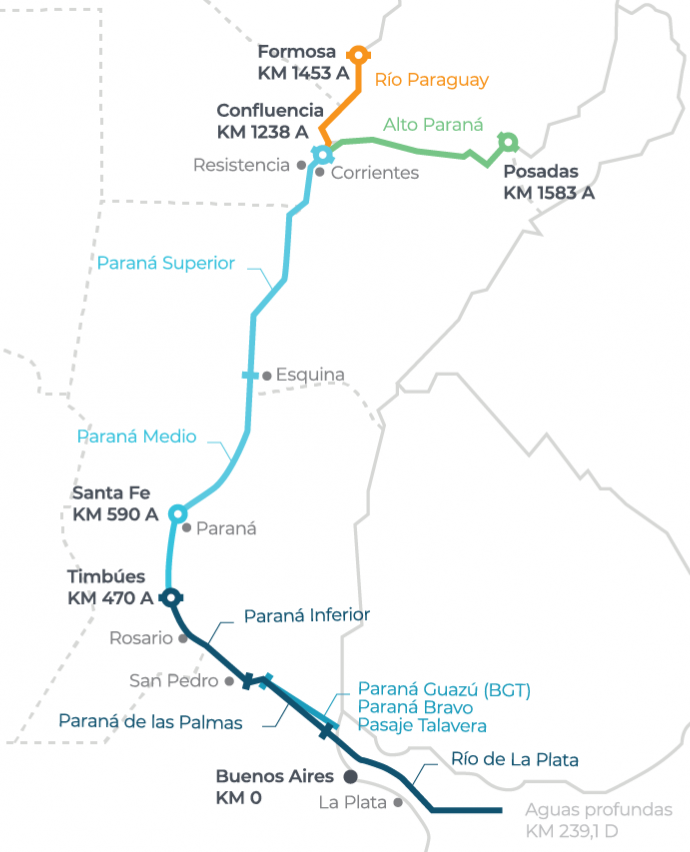
\includegraphics[width=0.5\linewidth]{figures/ch2/2025_mapa_vnt_extendida_tramos_profundidades_abril.png}
    \caption{The Vía Navegable Troncal (VNT) and the location of the Paraná Guazú in it \autocite{NavegableTroncal2025}}
    \label{fig:VNT}
\end{figure}

\section{Classification of Rio Paraná}

Rivers can be described and classified in different ways. This classification can be linked to several factors such as age, colour or seasonality. 

\subsection{The Age Classification of a River}
Based on the development of the channel stage of a river, it can be labeled as youthful, mature or old age.  \autocite{davisGeographicalCycle1899}
Applying this to the Rio Paraná makes it a complicated choice since the river is so long that it possesses features linked to each age label at distinct locations. therefore, it would be wiser to divide the Rio Paraná in three parts: upper, middle and lower Paraná. A youthful channel can be recognized through rapid flow, significant erosion, and a steep gradient. All these traits can be attributed to the upper Paraná zone.
Moving on, a mature channel stage of river is in most cases a developed floodplain in the form of loops, called 'meander', and lateral erosion. This is mostly what can be seen in the middle part of the Paraná river.
Lastly, the characteristics of an old age channel are comparable to the lower Paraná river. A wider floodplain, less rapid flow, and Deltas. All of this is explained in \autocite{orfeoParanaRiverArgentine2023}, and can be seen in the following figure from \autocite{lopezweibelSourcesTemporalDynamics2022}.



\begin{figure}[H]
    \centering    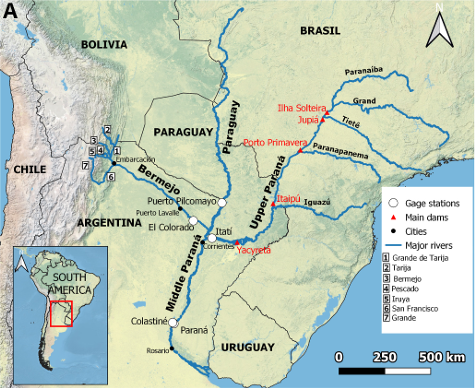
\includegraphics[width=0.5\linewidth]{figures/ch2/map rio parana.png}
    \caption{Rio Paraná Map}
    \label{fig:rio parana map}
\end{figure}


From Davis's study it makes sense that all these stages are represented in the total picture of the Paraná river since it is the ninth largest river in the world based on discharge \autocite{lopezweibelSourcesTemporalDynamics2022}.

\subsection{The Colour Classification of a River}
The colour of the river is also another label that can create a distinction. Based on two sets of papers/research  \autocite{furchWaterChemistryAmazon1984}, \autocite{sioliAmazonLimnologyLandscape1984}  Junk 1997, the water in rivers can be described as black, white or clear. The black water river is attributed to the 'leaching of tannins from decayed leaves of adjoining vegetated lands' \autocite{sand-mining-boek}, most comon in Amazonia or in the United States. White waters on the other hand are, contrary to its qualification, usually brown coloured due to the high sediment concentration. Clear water rivers are located in environments with little to no erosion.
Based on the theory and satellite imagery, one can again classify the Rio Paraná in different as a black and white river depending on the zone. The upper Paraná can be considered to be black due to its lack of sediment content, but rich in leaves content. But after the Bermejo river joins the Paraná, the river turns muddy all the way to the sea near Buenos Aires. \autocite{lopezweibelSourcesTemporalDynamics2022}

\begin{figure}[htbp]
    \centering
    \begin{subfigure}[b]{0.48\textwidth}
        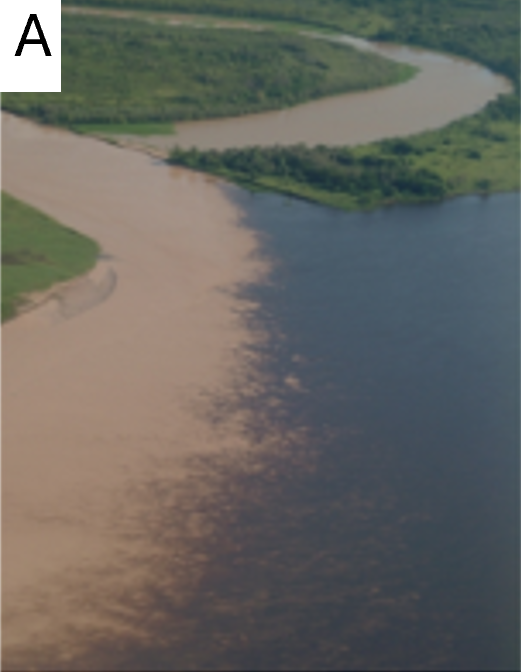
\includegraphics[width=\linewidth, height=5cm]{figures/ch2/Paraguay-Bermejo.png}
        \caption{Confluence of the Paraguay and Bermejo River}
        \label{fig:bermejo}
    \end{subfigure}
    \hfill
    \begin{subfigure}[b]{0.48\textwidth}
        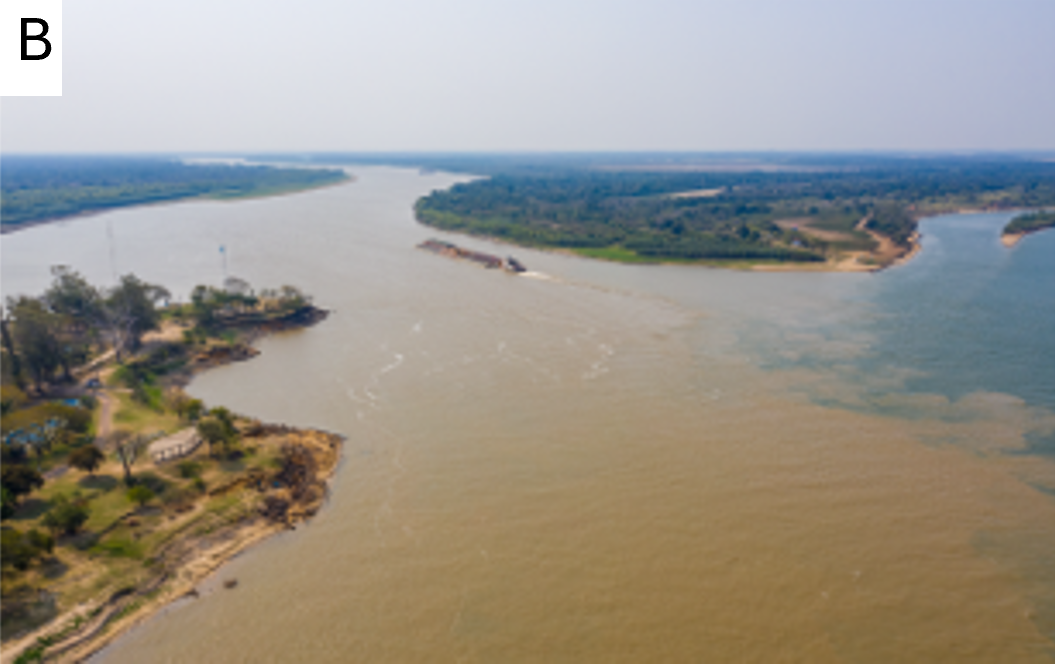
\includegraphics[width=\linewidth, height=5cm]{figures/ch2/Paraguay Parana.png}
        \caption{Confluence of the Paraguay and Paraná River}
        \label{fig:parana}
    \end{subfigure}
    \caption{Confluences of the Paraguay River with the Bermejo (left) and Paraná (right)}
    \label{fig:confluences}
\end{figure}

\subsection{The Seasonal Flow of a River}
The last classification relevant for this study is based on the flow characteristics and water availability. There are once again three types of categories: ephemeral, intermediate and perennial rivers. Ephemeral means that the river flow is not continuously present throughout the calendar year. Perennial rivers are the rivers whose flow is continuous and does not dry up during dry season, unlike the ephemeral rivers. Lastly the intermediate rivers are perennial rivers that dry up in extreme cases of drought.
The Rio Paraná can be considered a perennial river due to its continuous flow over the years \autocite{furchWaterChemistryAmazon1984}, \autocite{sioliAmazonLimnologyLandscape1984}.

\section{Origin of sediment content in Paraná Guazú}
\label{sec:origin sediment content}

A key step in constructing the sediment balance of the Paraná Guazú, located in the lower Paraná, is to identify the origin of its sediment. As shown in Figure \ref{fig:placeholder}, the lower and middle Paraná receive discharge from three main tributaries: the Bermejo, Paraguay, and upper Paraná rivers. The total average discharge in the middle Paraná is $18,389~\mathrm{m^3/s}$, of which 78\% is supplied by the upper Paraná. \citeauthor{lopezweibelSourcesTemporalDynamics2022} report that the Bermejo contributes only 2\% of this discharge. Nevertheless, the Bermejo is the dominant source of sediment, due to intense erosion in the Andes Eastern Mountain Range within its basin. During the wet season (November to April), multiple tributaries in the basin contribute large sediment flows, accumulating to an annual suspended sediment load of $106 ~\times 10^6$ t per year at El Colorado gauge station. 

It is interesting to know that the contribution of sediment from the Bermejo to the Paraná is approximately 90\% today, but that this is in fact due to the installation of the Itaipu dam built in 1971, located in the south of Brazil just before the border with Argentina and Paraguay. This modification of the sediment voyage cuts a supply of about 50\% compared the initial amount of sediment, this 90\% used to be 56\% of the sediment income before the construction of the dam. This explains us that the human action already hindered the initial inflow of sediment a long time ago \autocite{hibaParanaRiverEcological2024}.

In summary, while the Paraguay and upper Paraná rivers provide most of the fluvial discharge to the downstream delta, the Bermejo River delivers the majority of sediments (\cite{lopezweibelSourcesTemporalDynamics2022}). For this reason, the stretch of river beginning in the Bermejo basin and continuing via the Paraguay and middle Paraná to the Paraná Guazú is of particular importance in this study.  

\section{Mining of the Sand and Types of Dredging in a River}
Due to the need of sand in our society, various techniques have been established to get hold of the sand in the river beds. In this subpart the different dredging techniques will be explained.
For the sake of this study the focus will lie on in stream mining, the extraction of sand and gravel from the active channel of a river \autocite{sand-mining-boek}.

\textit{Bar scalping or skimming}:
This is the most common practice of extraction. It consists of taking away the two thirds of the bar, leaving the top third to minimize the alternation of the river bed initial conditions.

\textit{Dry pit channel mining}:
This method relies on using tools (mechanical or manual) to create a dry pit in which the sand or gravel can be extracted. The state in which the pits are left after extraction act has head cuts, altering the upstream flow during the high seasons.

\textit{Wet pit channel mining}:
Usually, the pit is made in a perennial river, but the effects and damages are the same as for the dry pit channel mining.

\textit{Bar excavation}:
This excavation process happens downstream of the bar, in order to get a hold of the sand and gravel going downstream.

\textit{Instream traps}:
For this excavation method a hole is dug so that the sediment gets caught during high season. This sediment can later be captured when the tides are low again.



\section{The effects of river sand mining}
\subsection{River bed}
As mentioned in the previous section, rivers maintain an equilibrium between erosion, transport, and deposition of sediments. However, instream sand mining can discrupt this balance. This happens through direct disruption of the channel geometry or through so-called incision and related undercutting of banks \autocite{sand-mining-boek}.

The direct disruption of the river bed depends on the type of sand mining technique employed. In the case of pit excavation, the river bed is locally lowered and a so-called 'nick point' is created. With bar skimming the river bed is widened \autocite{sand-mining-boek}. For the remainder of this section, the consequent effects of the local river bed lowering (the nick point) are discussed.

Channel incision causes the nick point to migrate both upstream and downstream. In the case of high flows, due to its shape, the nick point is the point where most erosion occurs. Water plunges over the step and erodes the bed at the base. As flows continue, the drop migrates upstream, a process which is often called head-cutting in literature. On the other hand, a process called 'hungry water' causes downstream migration of the pit \autocite{sand-mining-boek}.

A the mining pit the water level is deeper, which causes the flow velocity to reduce locally. This leads to a decrease in flow energy and thus to more deposited sediment. When the flow leaves the mining area, water levels are shallower again meaning that flow velocity and energy significantly increase. A lot of sediment has been deposited in the nick point, meaning that the water is not using its full sediment carrying capacity anymore. In other words, the water is 'hungry' for sediment and erosion downstream increases \autocite{sand-mining-boek}. 

Through the combined effects of head-cutting and hungry water, the mining pit can extend beyond the initial dimensions caused by direct disruption. This happens in both downstream and upstream directions, as summarized in figure \ref{fig:channelbedeffects}.

\begin{figure}[H]
    \centering
    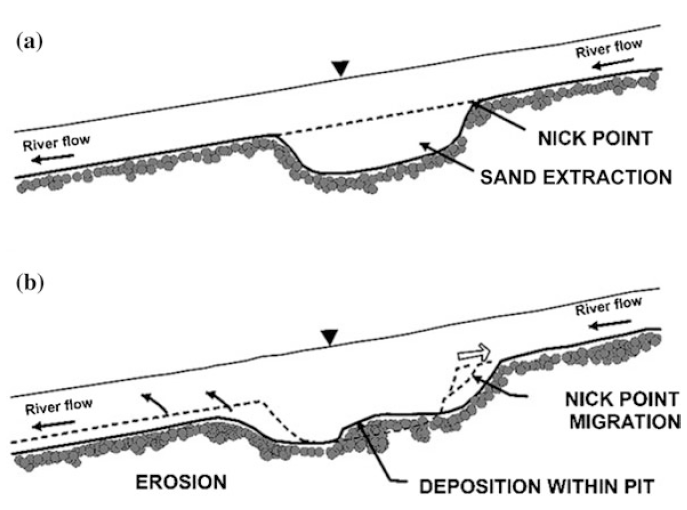
\includegraphics[width=0.75\linewidth]{figures/channelbedeffects.png}
    \caption{a: direct disruption leads to a locally lowered water bed, b: channel incision makes the pit migrate upstream through head cutting and downstream through 'hungry' water \autocite{sand-mining-boek}}
    \label{fig:channelbedeffects}
\end{figure}

\subsection{Sediment}
Previous studies have shown that bed coarsening can occur as a result of sand-mining. Fine particles are removed, leading to a greater concentration of coarse (gravelly) particles. This effect can also be seen upstream \autocite{sand-mining-boek}.

\subsection{Water quality and quantity}
Sand mining can lead to changes in both water quality and quantity. The process of dredging the fine sand stirs fine organic and inorganic particles, thereby increasing the turbidity of the water. This reduces light penetration, which means less photosynthesis and ultimately less organic growth in the water \autocite{sharipEffectsSeasonSand2014}.

As mentioned before, mining pits are often places with significant deposition of particles. Fine, nutrient-rich particles can settle and get trapped in the pits. This then reduces the transport of nutrients from the river to the coastal waters \autocite{sand-mining-boek}.

Concerning the water quantity, the most relevant effects are related to the groundwater: the lowering of the river bed through direct disruption or channel incision can lead to a lower groundwater table. This can lead to settlements or have negative effects on flora and fauna surrounding the river \autocite{rentierEnvironmentalImpactsRiver2022}.

\subsection{Biologic, socioeconomic and infrastructural changes}
The effects of sand mining can be diverse: previous studies have shown negative impacts on biodiversity, including reduced benthic fauna, disrupted fish spawning habitats, and depletion of natural mosquito predators such as dragonflies \autocite{sand-mining-boek}. The socioeconomic effects of mining can vary, in the short-term it often provides employment, income, and government revenue through royalties and taxation. However, in the long-term the operation can cause a reduction in access to clean water and can cause water scracity, especially in dry periods. Additionally, loss of land and access to land together with loss of trees and vegetation can jeopardize the local food security. Finally, infrastructure can be damaged by the lowering of the river bed and/or the groundwater table \autocite{sand-mining-boek}.

\section{Effect of tides and waves on the water level}
In addition to the study on the effects of sand mining on the river bed, it is as important to look at the effects of water on the river banks.

\subsection{Tides, waves and currents}
Relevant to this project, the two situations that contribute to this problem are the elevation of the water level due to the high astronomical tide, and the elevation of the water level/current due to the ship waves.

\textit{Astronomical tides}

The tides are the rise and fall of the water level, in particular the sea level, due to the gravitational force of the moon\autocite{usdepartmentofcommerceTidesCurrents}. As said, the tidal influence is the strongest in the ocean, pulling away the sea from one side of the globe to the other in function of the position of the moon, as seen in Figure 2.5.
\begin{figure}[H]
    \centering
    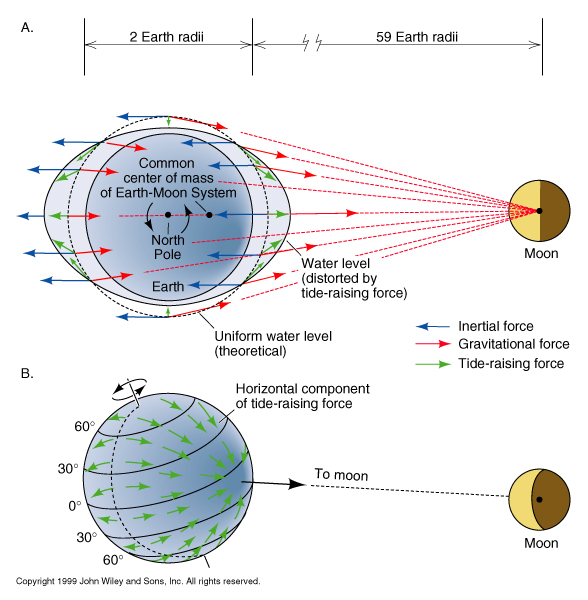
\includegraphics[width=0.5\linewidth]{figures/ch2/astronomical.jpg}
    \caption{Tidal movement due to gravitational force}
    \label{fig:placeholder}
\end{figure}
This gravitational force can also apply to rivers, as long as they are part of, or near a substantial quantity of water mass. Since the region of interest the  Rio Paraná Guazú and Ibicuy are quite near the delta of the Paraná and the river mouth, it is expected to be of significance for the data analysis. This will be treated in section \ref{sec 5.2 Hydrodynamic data}.

\textit{Waves}

The gravitational force not only yields a change in water level, but is also responsible for tidal waves. These are induced by the gravitational pull, in the direction of the moving current. 
In addition to that, there are also wind waves. These are produced by a striking distance called the fetch, where the wind blows on the surface of the water, gathering energy which translates into a wave. In order to find the significant wave height of this situation, one takes a sample of wave heights from buoys and takes the average of the three highest waves. (formula necessary??)

Given the fact that the river is not straight, the fetch or striking distance is usually quite short, as seen in Figure 1.1 \ref{Figure 1.1}. This means that the impact of the wind waves is probably quite small. This subject will also be treated in section \ref{sec 5.2 Hydrodynamic data}.

The last part of the waves that will be treated in this subsection are the ship waves. These are created when a ship passes by and pushes away the water to make way for the boat to go forward. This situation initiates three types of waves, primary, secondary, and propeller wash waves\autocite{}, as seen in Figure 2.6 below.
\begin{figure}[H]
    \centering
    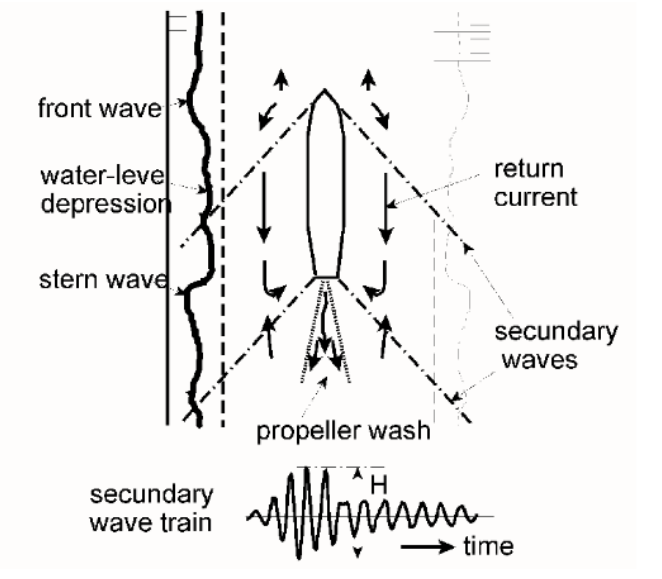
\includegraphics[width=0.5\linewidth]{figures/ch2/afbeelding.png}
    \caption{Ship Waves}
    \label{fig:placeholder}
\end{figure}
The impact of the secondary wave is the most promiscuous, as one can tell from the frequency plot underneath the sketch.



\textit{Correlated currents}

Due changes in water level as well as supplementary waves, a change in current applies. Using the standard values of the Netherlands and the given facts about the size of the ships circulating and the currents in the Rio Paraná Guazú, one could assume the wave height and current amplitudes for our case. This can be reflected once the field measures are known, in a later section \ref{Section 5}.
The table of the referencing values are as follows:

\begin{table}[H]
    \centering
    \caption{Standard values for wave heights and currents in the Netherlands (Data from CUR 197 ``Breuksteen in de praktijk'').}
    \label{tab:standard_values}
    \begin{tabular}{lcccc}
        \toprule
        \textbf{Location} & \multicolumn{2}{c}{\textbf{Wave heights (m)}} & \multicolumn{2}{c}{\textbf{Currents (m/s)}} \\
        \cmidrule(lr){2-3} \cmidrule(l){4-5}
        & \textbf{Wind waves} & \textbf{Ship waves} & \textbf{Natural current} & \textbf{Return current} \\
        \midrule
        Lakes          & 0.25 -- 1.00  & 0.10 -- 0.50  & 0.1 -- 0.5  & 0.1 -- 0.25 \\
        Canals         & 0.10 -- 0.25  & 0.25 -- 0.75  & 0.5 -- 1.0  & 0.5 -- 1.0  \\
        Rivers         & 0.25 -- 1.00  & 0.25 -- 0.75  & 1.0 -- 2.0  & 0.5 -- 1.0  \\
        Small waters   & 0.10 -- 0.20  & n.a.          & 0.2 -- 1.0  & n.a.       \\
        \bottomrule
    \end{tabular}
\end{table}


Understandably, the relevant row for this project is the 'River' category. Hinting to the fact that big ships are usually present in the channel, one might take values towards the upper boundary of the table.


\subsection{Effect on the river bed}

There are several ways how the water could have a negative impact on the river bank. In theory the river bank failure may be caused by house placement, water saturation, weight on the river bank, vegetation, and/or tectonic activity, but most of them due to the rise of the water level. The reason behind this is that the river bank is naturally eroded when the water exerts a force on it.
The river bank is divided in three parts: the toe, the bank and the overbank zone. The toe of the bank is the most susceptible to erosion when in contact with high water levels, which can be seen in the Figure 2.7 below \autocite{australiaRiverbankCollapse}.

\begin{figure}[H]
    \centering
    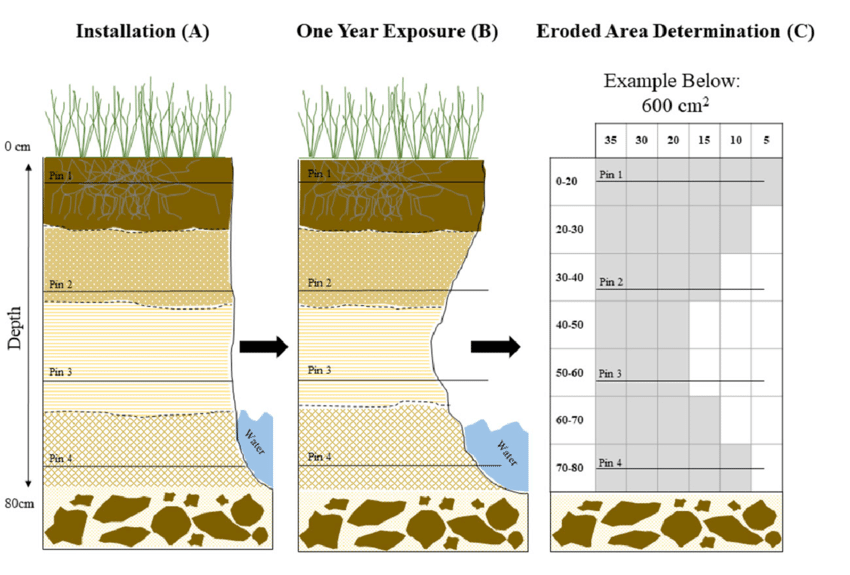
\includegraphics[width=0.5\linewidth]{figures/ch2/Erosion.png}
    \caption{Effect of Water on Bank after One Year}
    \label{fig:placeholder}
\end{figure}

When the combination of water level with a strong current is highest, the bank zone is affected by the tidal currents or waves. This is because, as seen in the Figure 7.2, water erodes the layer of the bank where the extra water level pushes, creating a dent inside the soil layer.
Consequently, after some time the upper overbank area has less and less support underneath, becoming thus unstable and partly falling down. 
Repeating this process takes the river bank further inside the land, increasing the channel width, absorbing the land of the local communities or agricultural fields that live near the river bank.

\section{Geotechnical background}
To understand more about the region and in order to be able to design mitigation measures in a later stage, the characteristics of the regional subsoil were researched. This section intends to combine all the available information regarding the subsoil in the investigation area.

\subsection{The geology of a delta}
A delta is a landscape formed at the mouth of a river where the water eventually runs into the ocean. At a delta, the water's velocity decreases which gives floating particles in the delta the change to settle. Among these floating particles are gravels, sands and clays, descending in particle size. The particles are formed by erosion of stone. The origin of the particles in the Parana river are the Andes mountains. 
Besides that, deltas are also characterized by high vegetation growth. When this vegetation dies, the organic material will change into peat due to the governing pressures. So, in a delta one expects to find relatively soft soils (sands) and very soft soils (clay and peat).

\subsection{Geological cross sections}
A study by \citeauthor{joseluiscavallottoEvolucionCambiosAmbientales2005} was conducted that led to a morphological map of the Paraná delta. In the study, for two cross sections a more detailed geological profile was made, one of which is relevant to the area of interest. The cross section along with the area of interest is shown in figure \ref{fig:crosssectiongeo}.

\begin{figure}[H]
    \centering
    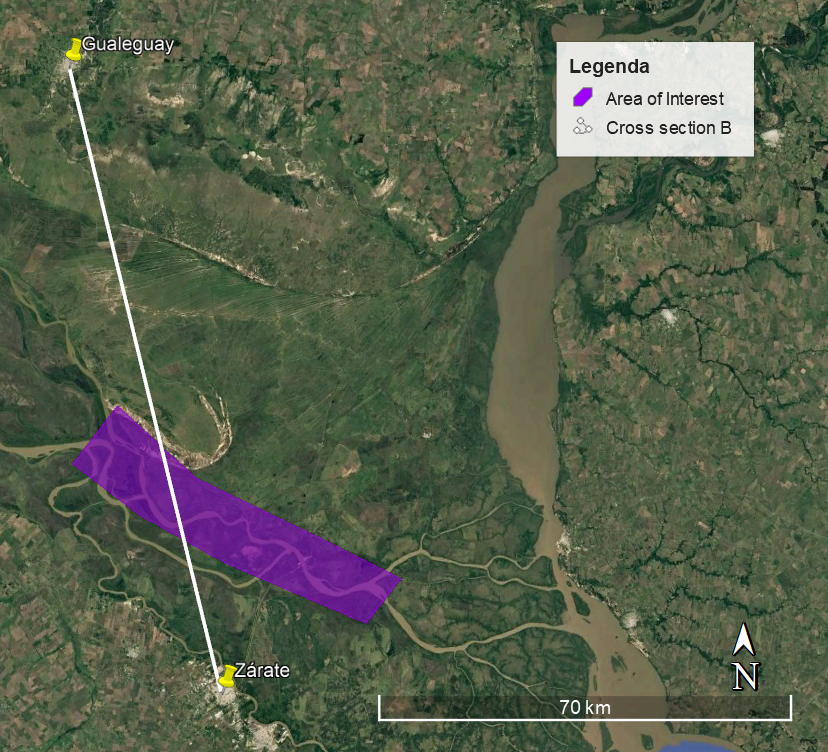
\includegraphics[width=0.75\linewidth]{figures/ch9/CrossSectionB.png}
    \caption{Cross section}
    \label{fig:crosssectiongeo}
\end{figure}

The geological profile of the cross section is shown in figure \ref{fig:geolprofile}. As can be seen in the figure, the taken cross section was around 80 km long. Of this, 15 km falls inside the area of interest, this zone is marked with purple.

\begin{figure}[H]
    \centering
    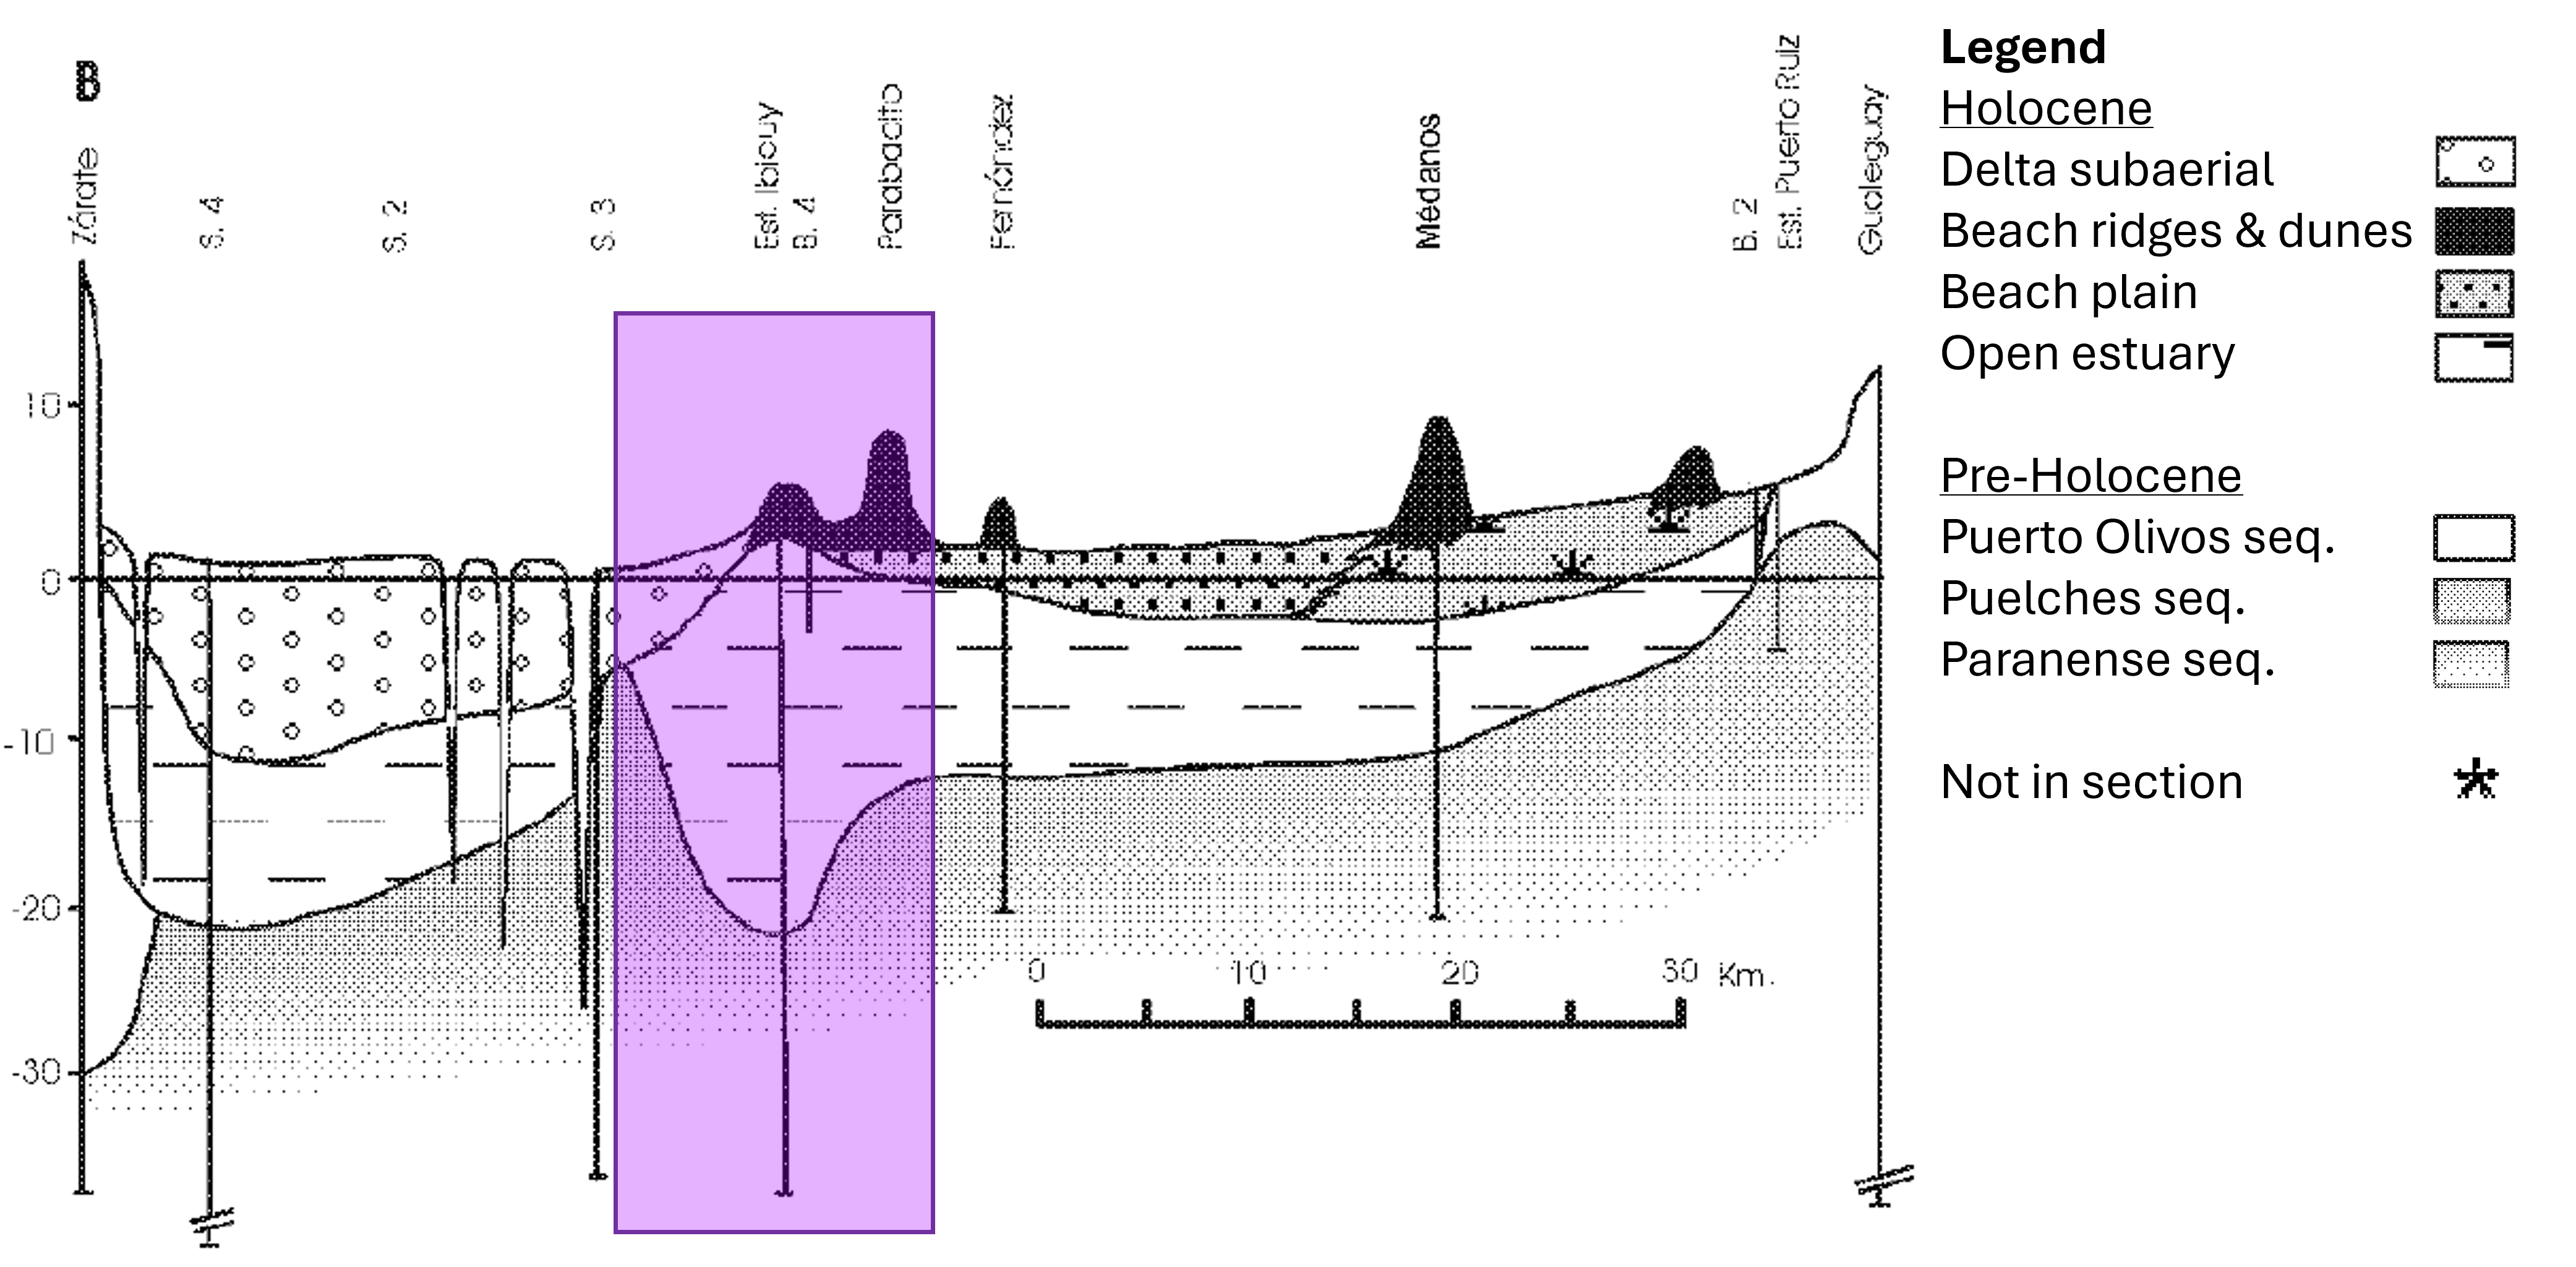
\includegraphics[width=1\linewidth]{figures/ch9/CrossSectionBResults.png}
    \caption{Geological profile of cross section \autocite{joseluiscavallottoEvolucionCambiosAmbientales2005}}
    \label{fig:geolprofile}
\end{figure}

In figure \ref{fig:geolprofile}, the first kilometers of the purple zone are especially of interest since these are located near the river. The following layers can be identified in this area.

\subsubsection{Subaerial facies}
The subaerial facies of the Paraná Delta developed through the deposition of silty-sandy sediments delivered mainly by the Paraná Guazú and Paraná de las Palmas \autocite{joseluiscavallottoEvolucionCambiosAmbientales2005}. These deposits occur at elevations between 2 m and sea level, with a maximum thickness of 12 m. This is the layer that is drained.

Mineralogical analyses show a predominance of quartz with minor plagioclase and K-feldspar, plus heavy minerals such as magnetite, hematite, garnet, zircon, tourmaline, and others, generally well-rounded except zircon, which preserves crystal form \autocite{rafaelcordiniContribucionConocimientoGeologia1949}. The age of the unit is debated: radiocarbon dates suggest origin dates between -150 BC and 180 AD, while other authors propose a later origin around 700–750 AD \autocite{joseluiscavallottoEvolucionCambiosAmbientales2005}.

\subsubsection{Open estuary}
The open estuary sediments were deposited during postglacial sea-level rise and were formed at the freshwater–saltwater interface during the upstream migration of the maximum salinity gradient, which filled the Río de la Plata river valley \autocite{joseluiscavallottoEvolucionCambiosAmbientales2005}.

These are olive-green clays to silty clays with thin fine-sand layers, scattered or concentrated shell beds, and fossil content confirming estuarine conditions. The unit is dated to the Holocene, with its base at ~6670 +/- 100 years BC, occurring between –22 and –0 m and reaching up to 20 m thick \autocite{vogelGroningenRadiocarbonDates1969}.

\subsubsection{Paranense depositional sequence}
During the Miocene, large portions of present-day Argentina, Uruguay, Paraguay, southern Brazil, and eastern Bolivia were covered by the Paranense Sea. This was a shallow sea that advanced from the Atlantic into the interior of South America . Its waters left behind extensive marine sediments and fossils and this layer is now known as the Paranense depositional sequence \autocite{tineoReconstructingSouthAmerican2024}.

It is composed mainly of siliciclastic sandstones, mudstones, and bioclastic beds, with thicknesses ranging from a few meters in outcrop to over 100 m. The lower part has mud-dominated offshore deposits with marine fossils, while the upper part shows sandier shoreface. Studies constrain the unit to the Late Miocene (ca. 9.5–6.7 Ma) \autocite{tineoReconstructingSouthAmerican2024}.

\subsubsection{Cross section by \citeauthor{amatoESTRATIGRAFIACUATERNARIASUBSUELO2009}}
Another study focuses on subsurface deposits from Diamante in Entre Ríos to San Fernando in the Buenos Aires province. Based on lithologic, clay mineral, radiocarbon, and outcrop data, the authors propose a depositional model for the region. This geological cross section is shown in figure \ref{fig:depmodel}. The purple area marks the area of interest for this research (Puerto Ibicuy).

\begin{figure}[H]
    \centering
    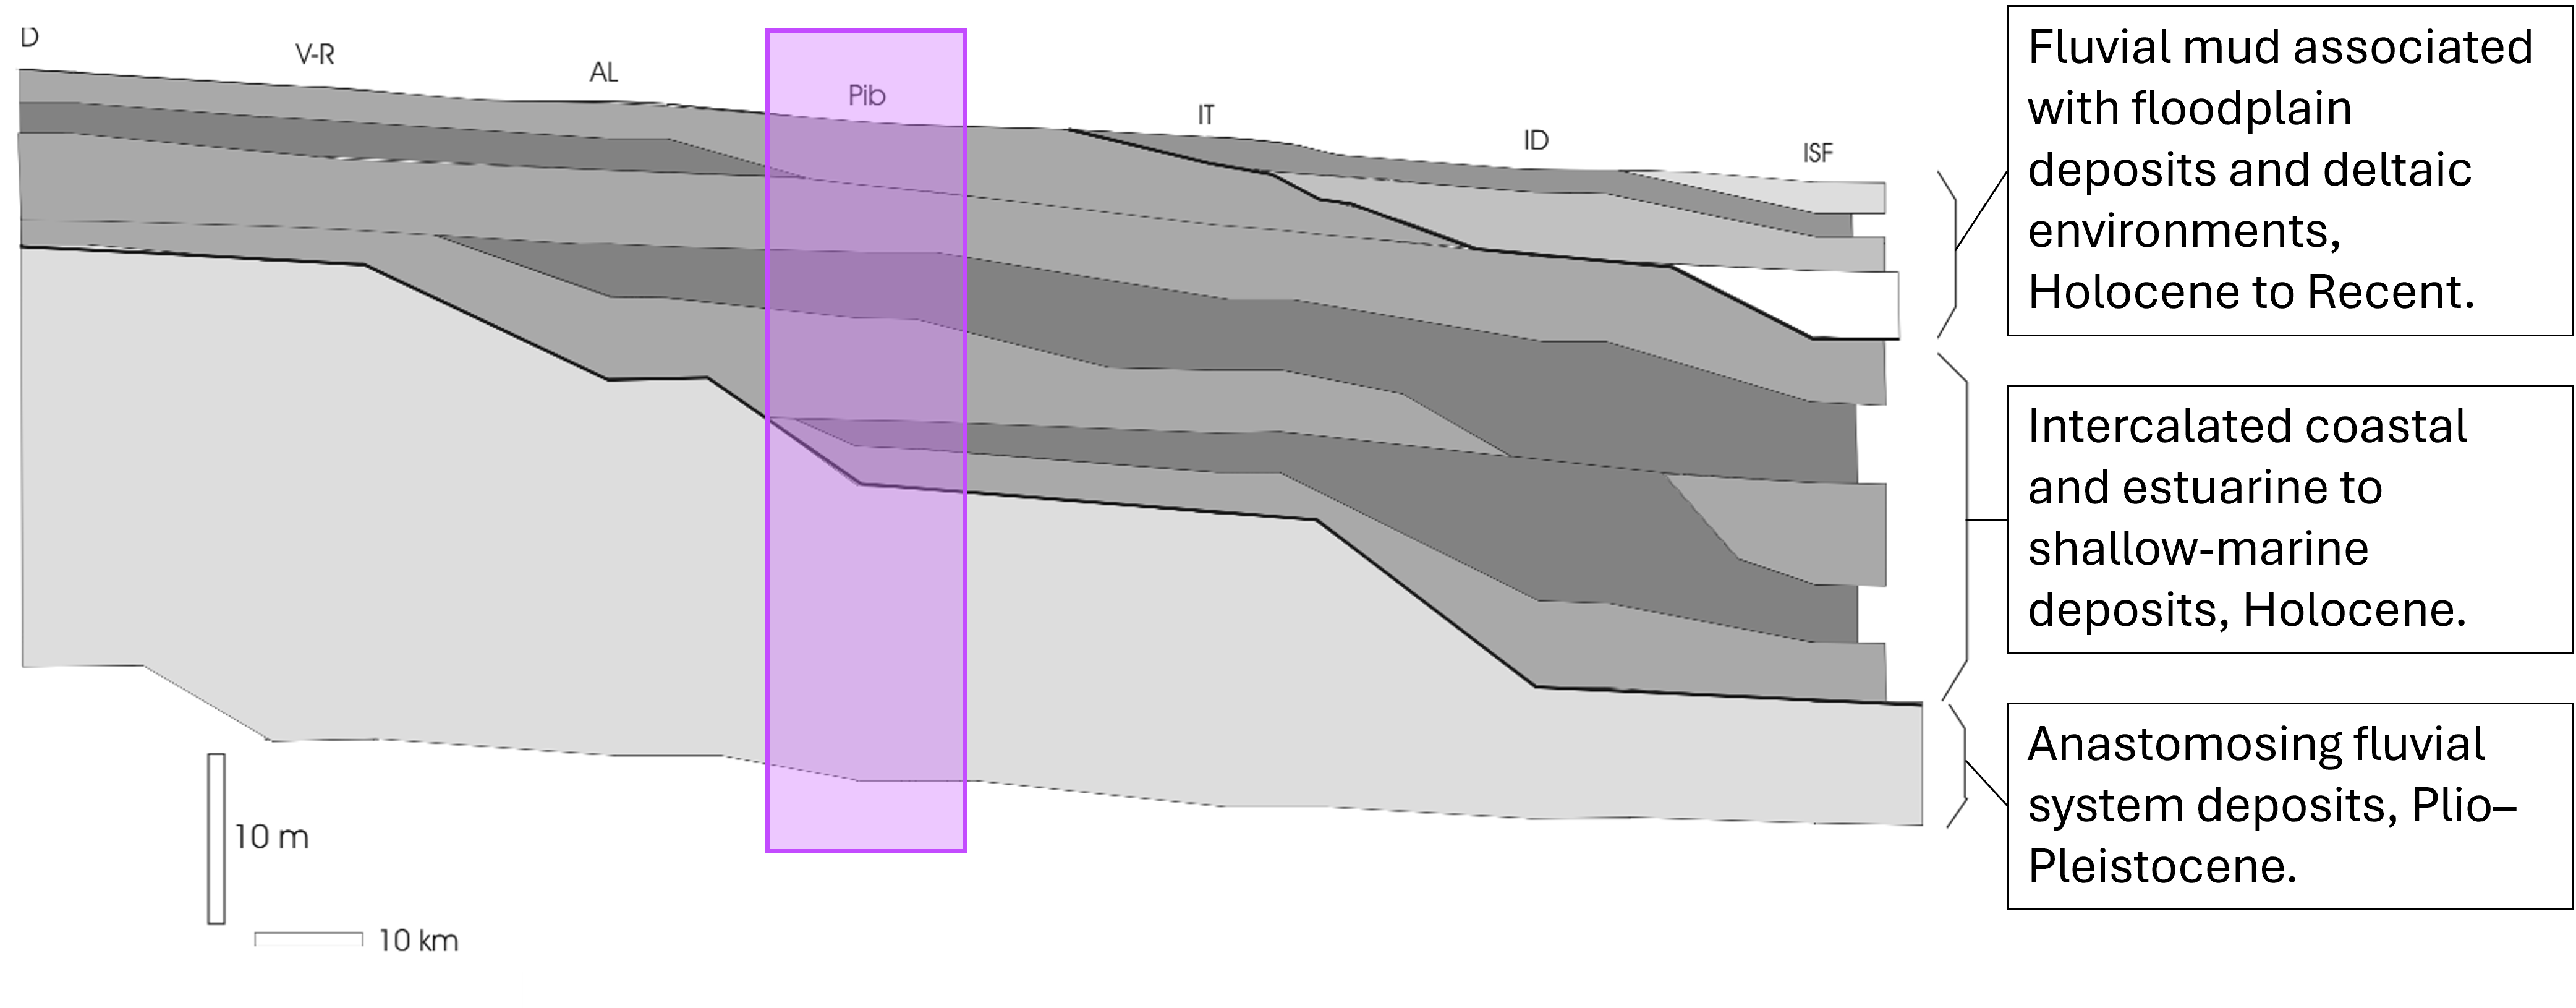
\includegraphics[width=1\linewidth]{figures/ch9/Crosssection2.png}
    \caption{Depositional model \autocite{amatoESTRATIGRAFIACUATERNARIASUBSUELO2009}}
    \label{fig:depmodel}
\end{figure}

As can be seen in the figure, the first layer consists of deltaic and flooplain deposits from the Holocene until recent times. This is in accordance with the geological profile as shown in figure \ref{fig:crosssectiongeo}. Underneath, holocene coastal/estuarine sediments can be found and below there are the Plio–Pleistocene fluvial deposits. The estuarine sediments can also be found in figure \ref{fig:crosssectiongeo}, but a different conclusion was reached for the final layer. \citeauthor{joseluiscavallottoEvolucionCambiosAmbientales2005} conclude that this is a pre-holocene marine deposit from the Miocene Paranense Sea, while here Plio–Pleistocene river deposits are placed below the Holocene sequence.

\section{Borehole}
In the same study conducted by \citeauthor{amatoESTRATIGRAFIACUATERNARIASUBSUELO2009}, a number of boreholes were executed along the lower Paraná \autocite{amatoESTRATIGRAFIACUATERNARIASUBSUELO2009}. One of these boreholes were executed near the area of interest in Puerto Ibicuy. The borehole was interpreted and with this the following soil profile was made  \autocite{amatoESTRATIGRAFIACUATERNARIASUBSUELO2009}.

\begin{figure}[H]
    \centering
    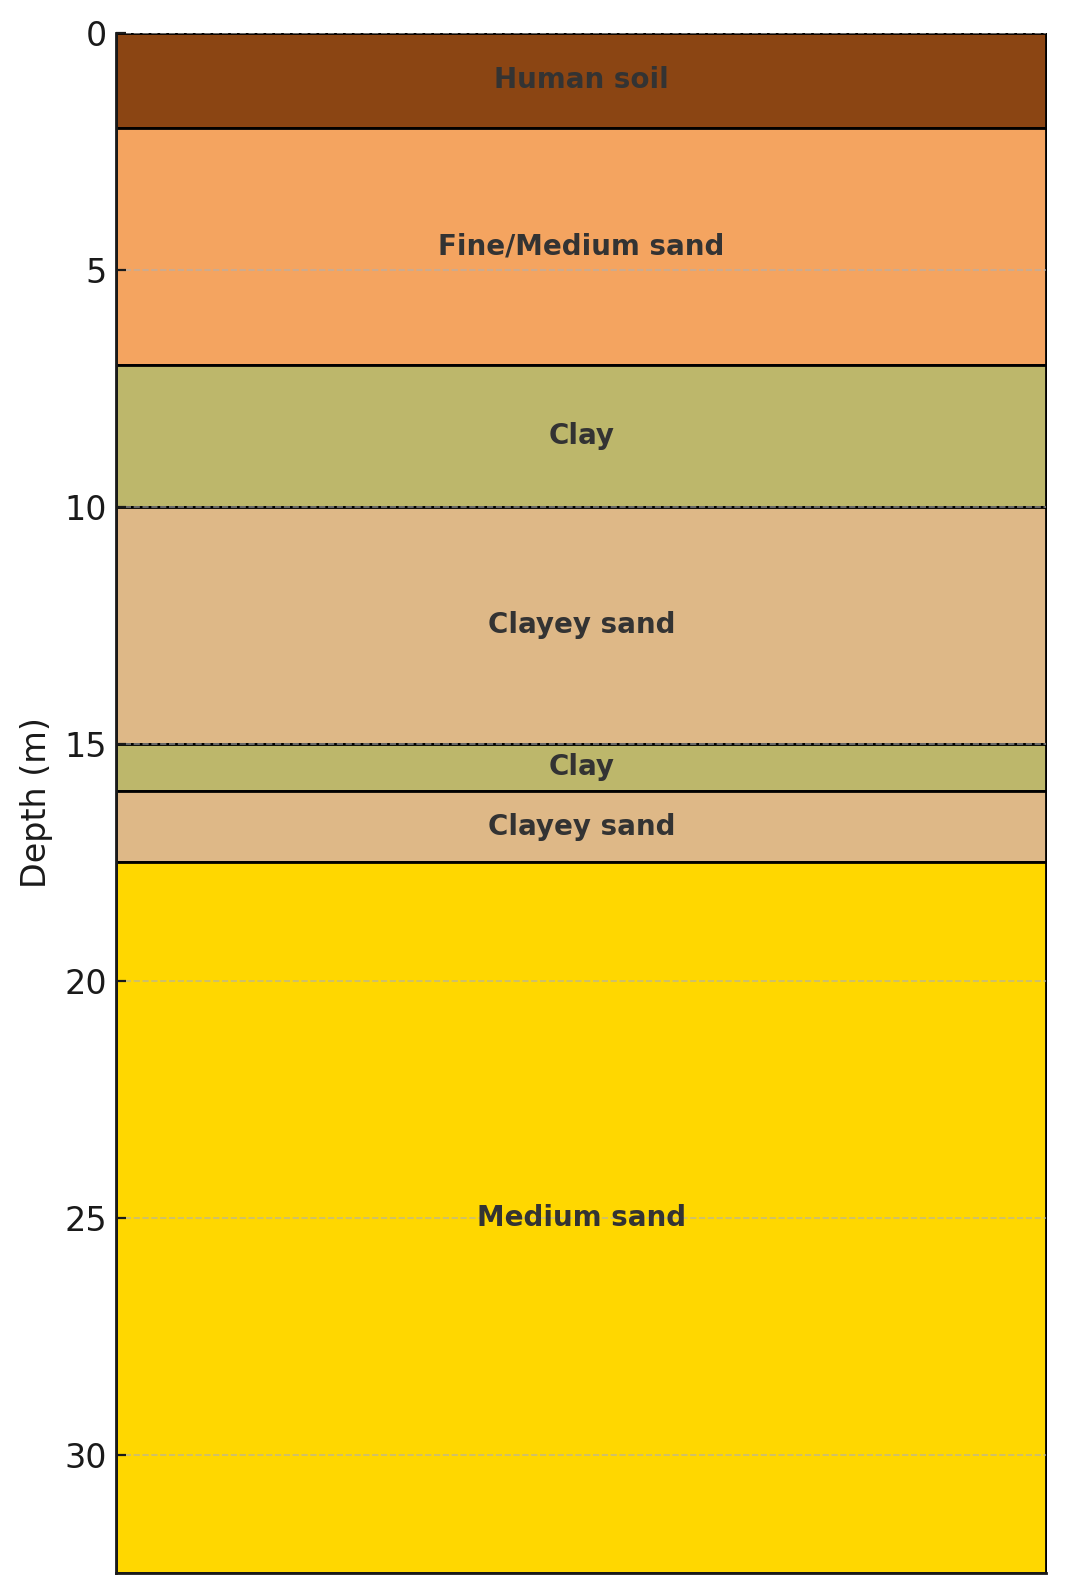
\includegraphics[width=0.45\linewidth]{figures//ch9/Bodemprofiel.png}
    \caption{Borehole profile in Puerto Ibicuy \autocite{amatoESTRATIGRAFIACUATERNARIASUBSUELO2009}}
    \label{fig:borehole}
\end{figure}

\section{Geotechnical summary}
To be able to design mitigation measures, the soil layers along with their geotechnical parameters should be known. For this, the borehole is deemed the most relevant source. The borehole shows a top layer with fine/medium sands. Below, clay/clayey sand can be found, and the bottom layer consists of medium sand. This is in accordance with the geological profiles that were provided before in figures \ref{fig:crosssectiongeo} and \ref{fig:depmodel}. Both frameworks describe a fluvial-to-estuarine-to-marine vertical transition. The top fluvial deposits help declare the presence of sandy deposits at the top and the layers of clay/clayey sand below correspond to estuarine deposits. Finally, old marine/fluvial deposits were likely compacted and lead to the layer of medium sand found at the bottom of the borehole.

Because of the resemblance between the local borehole and geological profiles given before, the layering as shown in figure \ref{fig:borehole} is deemed representative for the whole study area. Based on this layering the relevant parameters can be derived, the result in shown in table \ref{tab:soil_layers}.

\begin{table}[H]
    \centering
    \begin{tabular}{|c|c|c|c|c|c|c|c|}
        \hline
        Start layer (m) & End layer (m) & Soil type & \makecell{ $\gamma_d$ \\ (kN/m$^3$) } & \makecell{ $\gamma_{sat}$ \\ (kN/m$^3$) } & \makecell{ $\varphi'$ \\ ($^\circ$) } & \makecell{ $c'$ \\ (kPa) } & \makecell{ $c_u$ \\ (kPa) } \\
        \hline
        0 & 2 & Fill (Topsoil/Agricultural) & 12 & 12 & 15 & 2.5 & 20 \\
        2 & 7 & Fine/medium sand & 17 & 19 & 30 & 0 & - \\
        7 & 10 & Clay & 14 & 14 & 17.5 & 0 & 25 \\
        10 & 15 & Clayey sand & 18 & 20 & 25 & 0 & - \\
        15 & 16 & Clay & 14 & 14 & 17.5 & 0 & 25 \\
        16 & 17.5 & Clayey sand & 18 & 20 & 25 & 0 & - \\
        17.5 & 32 & Medium sand & 18 & 20 & 32.5 & 0 & - \\
        \hline
    \end{tabular}
    \caption{Soil stratigraphy and geotechnical properties.}
    \label{tab:soil_layers}
\end{table}

The parameters in table \ref{tab:soil_layers} were derived from the Eurocode \autocite{stichtingkoninklijknederlandsnormalisatieinstituutNederlandseNormNEN2025}. Because of limited knowledge on soil characteristics, conservatives estimates were made based on this code. In the borehole, no explicit information is given on the top fill layer. Therefore, conservative parameters are assumed based on typical values for organic topsoil.











